\section{Electron Energy Loss Spectroscopy}
\label{sec:eels}

A powerful technique to explore the local electronic properties
of nanoscale materials is electron energy loss spectroscopy 
within the transmission electron microscope.
%
As in all TEM-based method, in EELS an electron-transparent sample is illuminated by a 
beam of energetic electrons and then the scattered beam after crossing
the sample is focused by a magnetic prism
towards a spectrometer, thanks to which the distribution of energy losses $\Delta E$ can be recorded.
%
As schematic illustration of a typical EELS setup shown in the left panel of Fig.~\ref{fig:EELS}.

EELS spectra are divided into three main regions.
%
The first one is the zero-loss region, centered around $\Delta E=0$
and that contains the contributions from both elastic scatterings
as well as those from electrons that have not interacted with the
sample.
%
This region is characterised by the strong, narrow peak known as
the Zero Loss Peak (ZLP), which is much larger than the contribution
from inelastic scatterings.
%
The second region is the low-loss region, defined as that for energy losses
$\Delta E \lsim 50$ eV, and which contains important information
about features of the studied sample such as plasmons, excitons, phonons, and
intra-band transitions.
%
Of particular relevance in this context is the ultra-low loss region, characterised by $\Delta E \simeq$ few eV,
where the contributions of the ZLP and that from the inelastic scatterings
off the sample partially overlap.
%
Finally, for $\Delta E \gsim 50$ eV one has the core-loss region,
which is used to provide compositional information
on the materials that constitute the sample.
 
%%%%%%%%%%%%%%%%%%%%%%%%%%%%%%%%%%%%%%%%%%%%%%%
\begin{figure}[t]
    \centering
    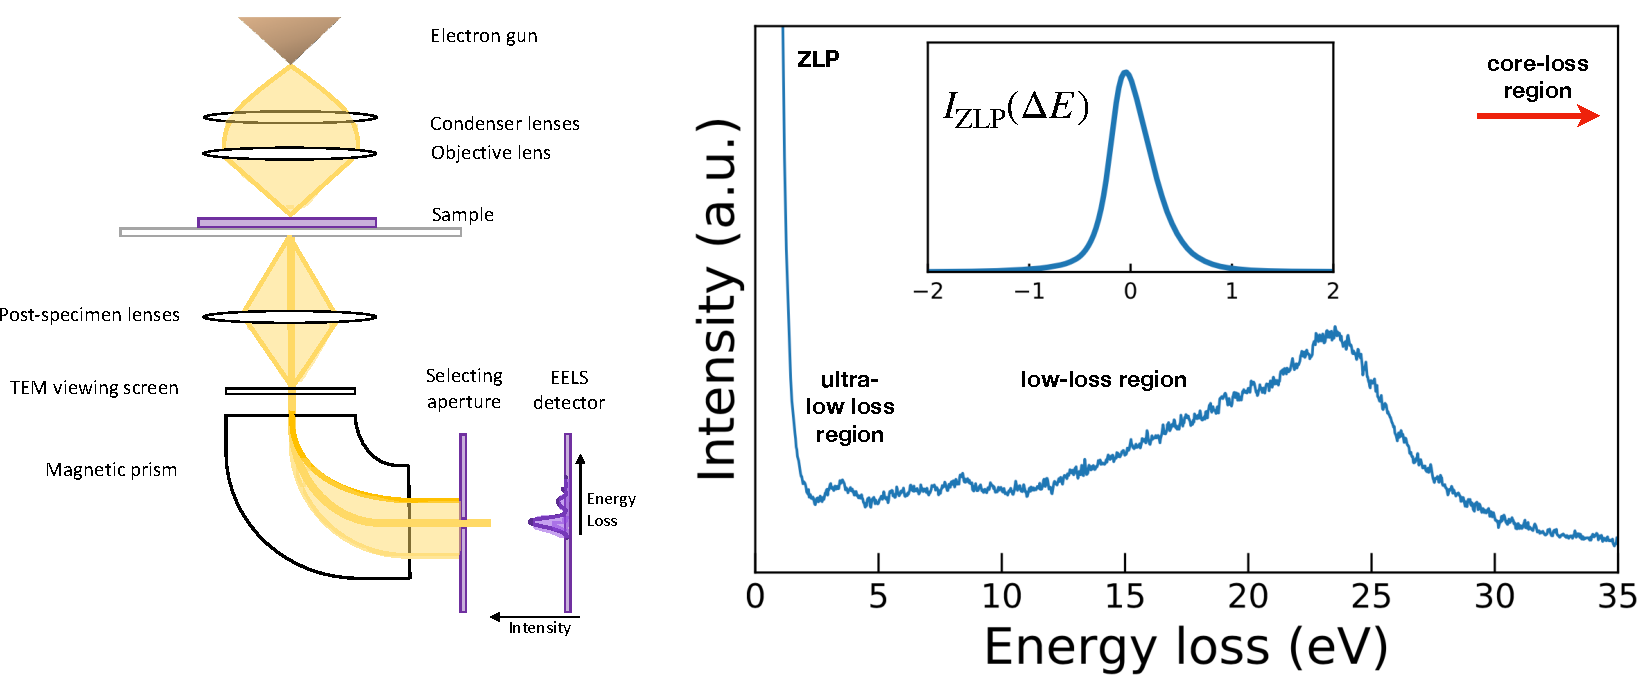
\includegraphics[width=0.9\textwidth]{plots/EELS.pdf}
    \caption{Left: in electron energy loss spectroscopy, a magnetic
      prism is used to deflect the electron beam that has crossed the sample
      in a way that the distribution of electron energy losses $\Delta E$ can be recorded
      by a spectrometer.
      Right: a representative EELS spectrum in the region $\Delta E \le 35$ eV, recorded
      on one of the WS$_2$ nanostructures presented~\cite{SabryaWS2}.
      %
      The inset displays the Zero Loss Peak, illustrating how
      its magnitude is larger than the contribution from the signal by several
      orders of magnitude.
      }
    \label{fig:EELS}
\end{figure}
%%%%%%%%%%%%%%%%%%%%%%%%%%%%%%%%%%%%%%%%%%%%%%%%5

The right panel of Fig.~\ref{fig:EELS} displays
a representative EELS spectrum in the region $\Delta E \le 35$ eV, recorded
on one of the WS$_2$ nanostructures presented~\cite{SabryaWS2}
and which will be further discussed in Sect.~\ref{sec:tmd}.
%
The inset displays the Zero Loss Peak, illustrating how
its magnitude is larger than the contribution from the inelastic scatterings
off the sample by several
orders of magnitude.
%
Clearly, carefully disentangling these two contributions in the region $\Delta E \simeq$ few eV
is essential for the physical interpretation of EEL spectra in the ultra-low-loss region.
%
The magnitude and shape of the ZLP intensity is known to depend not only on the specific values
of the electron energy loss $\Delta E$, but also in other operation parameters
of the TEM such as the electron beam energy $E_{\rm beam}$ and the exposure time
$T_{\rm exp}$, the aperture width and the use of a monochromator. 
%
This means that in general one cannot measure the ZLP for a given operation
conditions, say a high beam voltage of $E_{\rm b}=200$ keV, and expect to reproduce
the ZLP associated to different conditions, such as a  high beam voltage of $E_{\rm b}=60$ keV,
without introducing a specific model.
%
Several attempts to model the ZLP peak have had some success at fitting the main intensity of the peak, 
but in the tails discrepancies are as large as 25-35\%~\cite{Bangert:2003}.
%
The standard background 
subtraction method is to fit a power law to the tails, however this subtraction is not suitable in
many circumstances and regimes~\cite{Hachtel:2018, Tenailleau:1992, Reed:2002, Bosman:2006}.
%
Unfortunately, it is not possible to compute the dependence of the ZLP on $\Delta E$
and the rest of operation parameters of the microscope from first principles.
%
Further, even for identical operation conditions the value of the ZLP
will in general vary due to {\it e.g.} external perturbations such as electric or magnetic fields~\cite{Rafferty:2000},
the stability of the microscope and spectrometer electronics~\cite{Kothleitner:2003}, the local
environment (possibly exposed to mechanical vibrations and pressure and temperature fluctuations) 
and spectral aberrations\cite{Egerton:1996, Scherzer:1949}. 
%
Any model for the ZLP should thus account for this irreducible source of uncertainties.
%
In this work we will investigate EELS measurements collected  on a cold field emission gun JEOL
transmission electron microscope operating at different beam energies $E_{\rm beam}$
and equipped with a  Gatan spectrometer.
%
The energy resolution is of these measurements,
defined as the FWHM of the ZLP, is $\delta E=40$ meV.
%
These measurements have a spatial resolution of ...

%%%%%%%%%%%%%%%%%%%%%%%%%%%%%%%%%%%%%%%%%%%%%%%%%%%%%%%%%%
%%%%%%%%%%%%%%%%%%%%%%%%%%%%%%%%%%%%%%%%%%%%%%%%%%%%%%%%%%
